\section{Purpose of the laboratory work}

\begin{itemize}
	\item Obtaining testing skills for the functionalities of a software; 
	
	\item Forming abilities of partitioning input data in equivalence classes;
	
	\item Using decision tables and state/transition diagram to create test cases;
\end{itemize}

\section{Laboratory Work Requirements}
\begin{itemize}
	\item Elaborate a scenario of testing for 2-3 functionalities of an application;
	
	\item Determine organizational criteria of equivalence classes and decision tables;
	
	\item Develop a conclusive test according to the criteria including boundary testing;
	
	\item Emphasize test cases on which you can get error results;
	
	\item Make a report of the laboratory work;
\end{itemize}

\section{Intro to the technique}

In black-box testing, the purpose is to the test the different functionalities of an application without looking into the internal structure of the program. 

There are different strategies to use in order to test efficiently. 

For example equivalence class partitioning (ECP), decision tables and boundary-value analysis (BVA).

A graphical representation is in the following figure : 

\begin{center}
	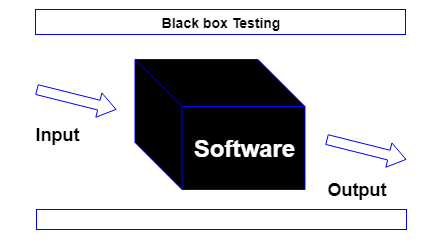
\includegraphics[scale=1]{images/Capture1}
\end{center}

\clearpage